\documentclass[mathserif]{beamer}
\usepackage{epstopdf}
\usepackage{amsmath}
\usepackage{helvet}
\usepackage{listings}
\usepackage{algorithm2e}
\usetheme{CambridgeUS}
%\usecolortheme{whale}


\title[Signal Parameter Estimation] % (optional, only for long titles)
{\textbf{Parameter Estimation of Complex Sinusoids in White Gaussian Noise}}
%\subtitle{Subtitle}
\author[Anchieta, Gendron] % (optional, for multiple authors)
{David Anchieta \and Advisor: Paul J. Gendron}
%\institute[UFPA UMassD] % (optional)
%{
% \inst{1}%
%  College of Computer and Telecommunications Engineering\\
%  Federal University of Para
%  \and
%  \inst{2}%
%  Department of Electrical and Computer Engineering\\
%  University of Massachusetts Dartmouth
%}
\subject{Digital Signal Processing}

\begin{document}
	\frame{\titlepage}

	\section*{Outline}
	\begin{frame}{Outline}		
		\tableofcontents
	\end{frame}
	
	%========================================================================
	%FIRST SECTION STARTS HERE
	%========================================================================
	\section{Single tone case}
	\begin{frame}{Estimating frequency and amplitude of a single tone}
		Given a complex sinusoid defined by:
		\begin{equation*}
			r(t) = A_{1}e^{j2\pi f_1 t} + z(t)
		\end{equation*}
		Where $z(t)$ is a complex Gaussian white noise with zero mean and variance $\sigma^2$.
		
		Givens a set of samples from $r(t)$, how could we estimate the values of $A_1$ and $f_1$?
		
		
		
		% \begin{figure}
			% \centering
			% \includegraphics[scale=0.35]{../img2/fig1.eps}
		% \end{figure}
	\end{frame}
	
	
	\subsection{Maximum likelihood estimators of frequency and amplitude}
	
	\begin{frame}{Note on Maximum Likelihood Estimation \#1}
		\begin{itemize}
			\item It's a method to estimate parameters of a statistical model.
			\item The value of the Maximum Likelihood Estimator of a parameter must make the observed data more likely.
		\end{itemize}
		\pause
		An example of maximum likelihood estimator: The sample mean of a set of $n$ observations from a random variable $X$.
		\begin{gather*}
			M_n = \frac{1}{n}\sum_{i=1}^nX_i\\
			\only<3->{ \lim_{n \to \infty}M_n = \mathrm{E}\{X\}}
		\end{gather*}
	\end{frame}
	
	\begin{frame}{Estimating frequency and amplitude of a single tone}
		We must chose a frequency that will maximize $\mathrm{p}(\mathbf{r}|f_1,A_1)$
		\begin{gather*}
			\mathrm{p}(\mathbf{r}|f_1,A_1) = \frac{1}{\pi^N\sigma^{2N}}\exp\left[-\frac{(\mathbf{r}-A_1\mathbf{e_1})'
				(\mathbf{r}-A_1\mathbf{e_1})}{\sigma^2}\right] \\	
			\mathbf{r} = A_1\mathbf{e_1} + \mathbf{n} \\
			\mathbf{e_1} =  [e^{j2\pi f_10} \; e^{j2\pi f_1T_s} \; \dots \; e^{j2\pi f_1(N-1)T_s}]^T 			
		\end{gather*}
		
		So we need to minimize
		\begin{gather*}
		(\mathbf{r}-A_1\mathbf{e_1})'(\mathbf{r}-A_1\mathbf{e_1}) = \mathbf{r'r}+A_1N-A_1\mathbf{r'e_1}-A_1\mathbf{e_1'r}
		\end{gather*}
	\end{frame}
	
	\begin{frame}{Estimating frequency and amplitude of a single tone}
		\begin{figure}
			\centering
			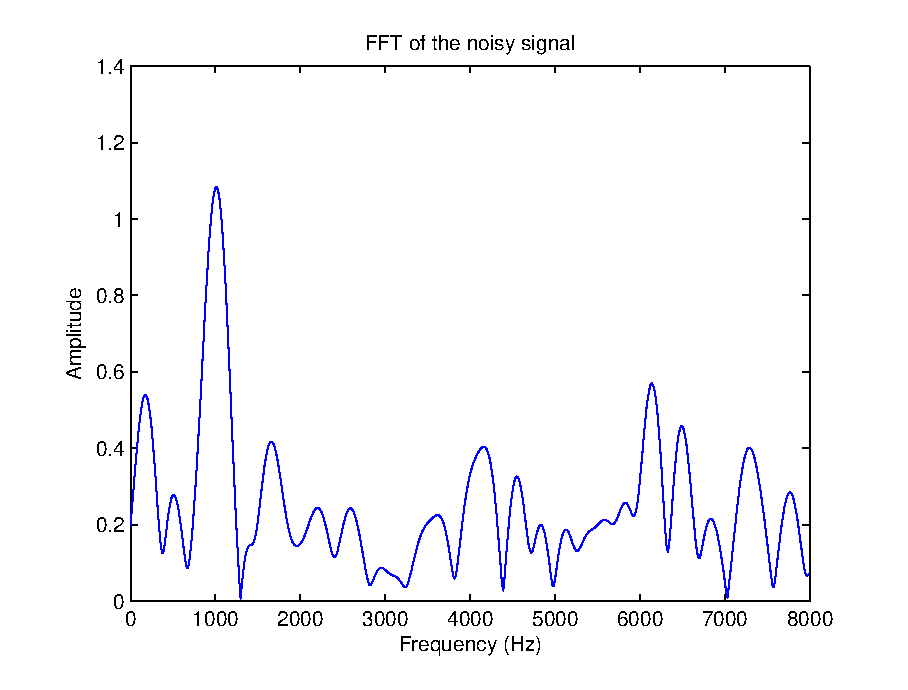
\includegraphics[scale=0.375]{../img3/singleTonewoMHFig2.eps}
			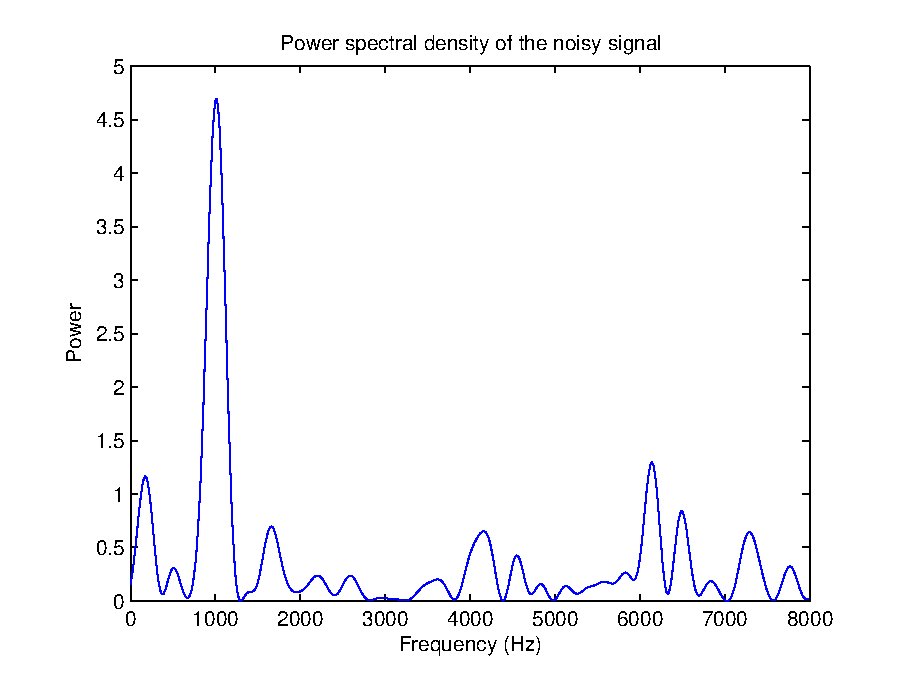
\includegraphics[scale=0.375]{../img3/singleTonewoMHFig3.eps}
			\caption{Discrete-time Fourier Transform and power spectral density of the signal with added noise.}
		\end{figure}
	\end{frame}
	
	\begin{frame}{Estimating frequency and amplitude of a single tone}
		The frequency can be easily estimated by picking the value at the peak of the spectrum of the signal.
		
		Knowing the MLE of the frequency, the estimate of the amplitude is given by the following equation.
		
		\begin{equation*}
			\hat{A}_1 = \left|\frac{1}{N} \sum_{n=0}^{N-1} r(nT_s)\exp{(-j2\pi \hat{f}_1nT_s)} \right|
		\end{equation*}
	\end{frame}
	
	\begin{frame}{Note on Maximum Likelihood Estimation \#2}
		Though the MLE is trustworthy, it has some limitations.
		\begin{itemize}
			\item The value doesn't have a probability related to itself neither intervals of confidence.
			\item It also doesn't decide if the signals has one or two tones.
			\item It can be less precise depending on the length of the data and signal-to-noise ratio.
		\end{itemize}
		Some of this problems are solved by computing a PDF of the parameters instead of just getting MLE's.
	\end{frame}
	
	\begin{frame}{Note on Maximum Likelihood Estimation \#2}
		\begin{figure}
			\includegraphics[scale=0.5]{../img3/mlefig.eps}
			\caption{An example of two parameters with the same maximum likelihood estimator.}
		\end{figure}
	\end{frame}
	
	% \begin{frame}{Estimating frequency and amplitude of a single tone}
		% \begin{figure}
			% \centering
			% \includegraphics[scale=0.45]{../img2/fig4.eps}
			% \caption{Histogram of the frequency and amplitude MLE after running the algorithm 10000 times.}
		% \end{figure}
	% \end{frame}
	
	%========================================================================
	%I START TO TALK ABOUT PDF'S HERE
	%========================================================================
	\subsection{Computing probability density functions}
	\begin{frame}{Defining the PDF of the frequency}
		Being $N$ the number of samples and $T_s$ the sampling period $1/f_s$, we have.
		\begin{gather*}
			\mathbf{r} =  [r(0) \; \; r(T_s) \; \; r(2T_s) \; \dots \; r((N-1)T_s)]^T \\
			\mathbf{e_1} =  [e^{j2\pi f_10} \; e^{j2\pi f_1T_s} \; \dots \; e^{j2\pi f_1(N-1)T_s}]^T \\		
			\mathbf{r} = A_1\mathbf{e_1} + \mathbf{n} \\
			\mathrm{p}(\mathbf{r}|f_1,A_1) = \frac{1}{\pi^N\sigma^{2N}}\exp\left[-\frac{(\mathbf{r}-A_1\mathbf{e_1})'
				(\mathbf{r}-A_1\mathbf{e_1})}{\sigma^2}\right] \\
			\mathrm{p}(\mathbf{r}|A_1) = \int \mathrm{p}(\mathbf{r}|f_1,A_1)\mathrm{p}(f_1)df_1\\
			\mathrm{p}(f_1|\mathbf{r},A_1) = \frac{\mathrm{p}(\mathbf{r}|f_1,A_1)\mathrm{p}(f_1)}{\mathrm{p}(\mathbf{r}|A_1)} \\
		\end{gather*}
	\end{frame}
	
	\begin{frame}{Defining the PDF of the frequency}
		\begin{figure}
			\centering
			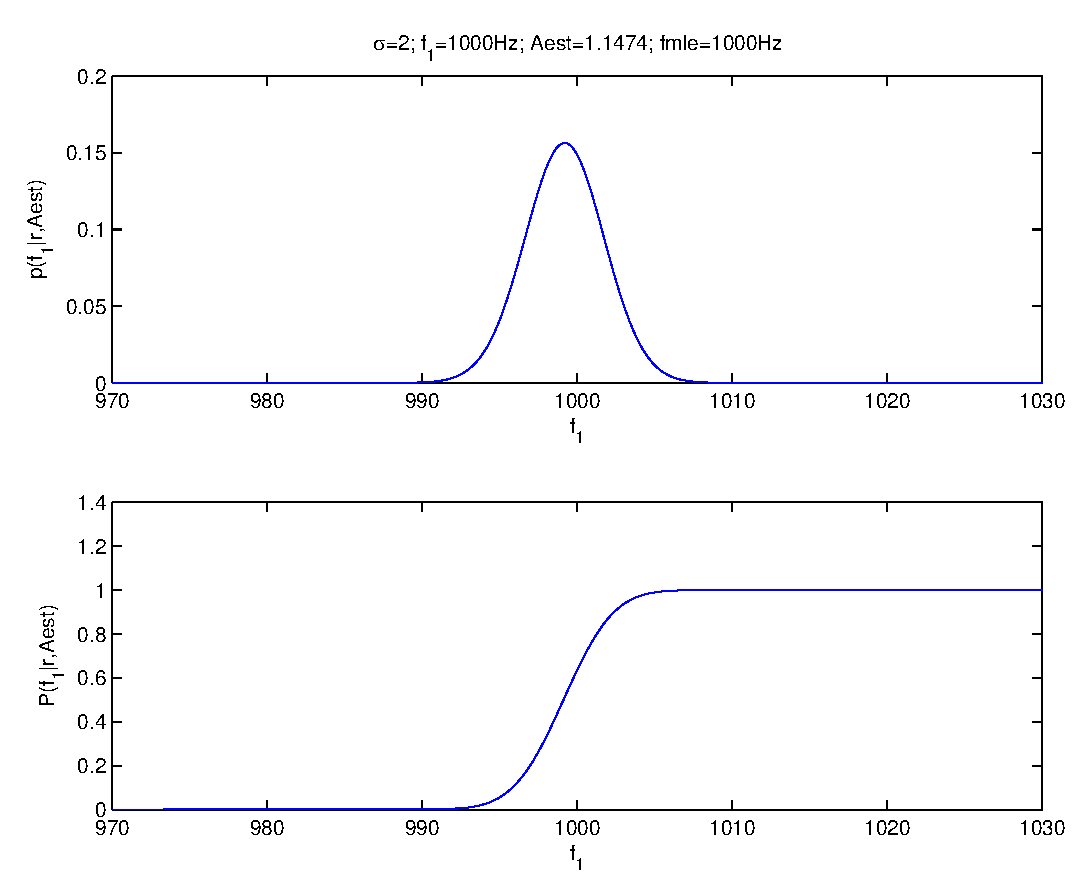
\includegraphics[scale=0.345]{../img3/singleTonewoMHFig11.eps}
			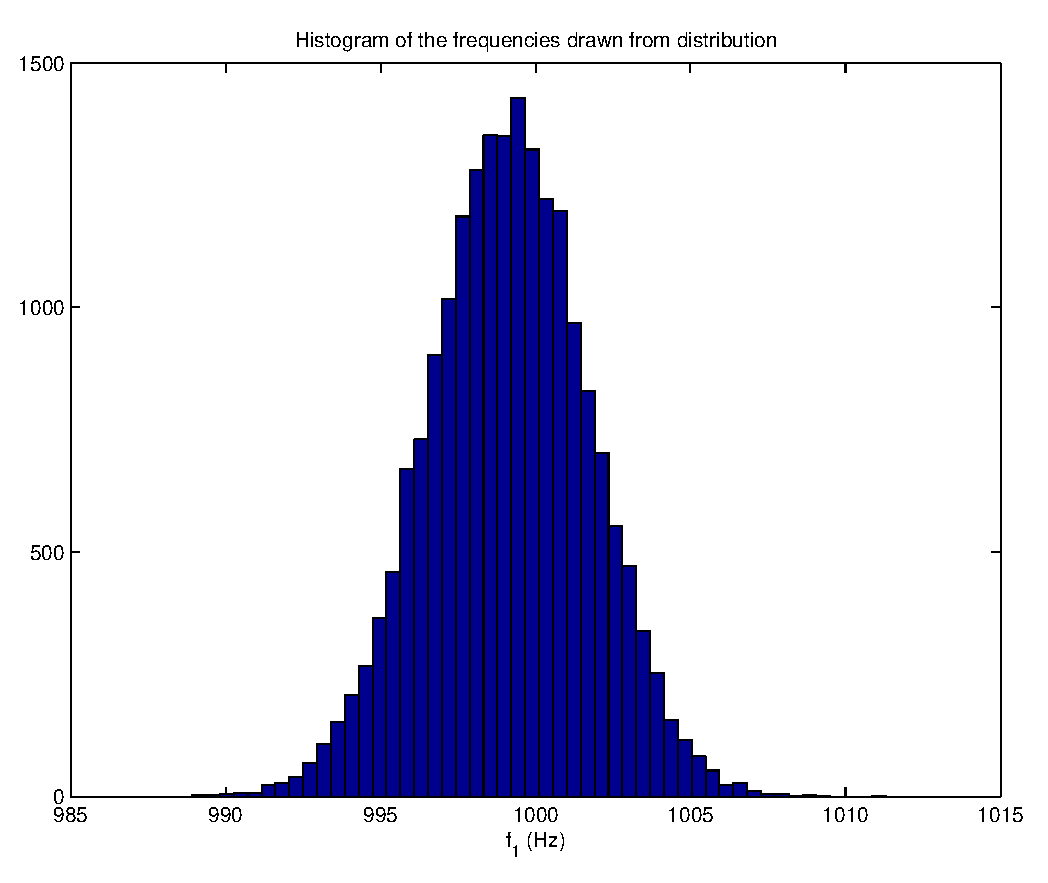
\includegraphics[scale=0.345]{../img3/singleTonewoMHFig12.eps}
			\caption{PDF of the frequency conditioned on the MLE of the amplitude.}
		\end{figure}
	\end{frame}	
	
	\begin{frame}{Defining the PDF of the amplitude}
		The PDF of the amplitude conditioned on a frequency $f_1$ is derived below.
		\begin{gather*}
			\mathbf{r} =  A_1\mathbf{e}+\mathbf{n}\\
			\mathbf{e'r} =  A_1N+\mathbf{ne}' \\
			A_1 = \frac{\mathbf{e'r}-\mathbf{n}\mathbf{e}'}{N} \\			
			A_1|\mathbf{r},f_1  \sim \mathcal{N}\left(\frac{\mathbf{e'r}}{N},\frac{\mathbf{e'I}\sigma^2\mathbf{e}}{N^2}\right) \\			
			A_1|\mathbf{r},f_1 \sim \mathcal{N}\left(\frac{\mathbf{e'r}}{N},\frac{\sigma^2}{N}\right) \\
			\mathrm{p}(A_1|\mathbf{r},f_1) = \frac{1}{\sqrt{\pi\sigma^2/N}}\exp\left[-\frac{(A - \frac{\mathbf{e'r}}{N})^2}{\sigma^2/N}\right]
		\end{gather*}		
	\end{frame}
	
	\begin{frame}{Defining the PDF of the amplitude}
	Since the estimate of the amplitude will be a complex random variable, its PDF needs to be plotted on a 2D Plane.
		\begin{figure}
			\centering
			\includegraphics[scale=0.35]{../img3/singleTonewoMHFig13.eps}
		\end{figure}
	\end{frame}
	
	%========================================================================
	%THE NEW SLIDES FOR THE JULY 7TH PRESENTATION START HERE
	%========================================================================
	\subsection{Joint PDF of frequency and amplitude}
	\begin{frame}[fragile]
		\frametitle{Algorithm to draw samples from joint PDF of amplitude and frequency}
		\begin{algorithm}[H]
			\For{n = 2:Nmcmc}{
			Asamp[n] = Sample of $A_1$ conditioned on fsamp[n-1];\\		
			fsamp[n] = Sample of $f_1$ conditioned on Asamp[n];\\
			}
		\end{algorithm}

\end{frame}
	
	\begin{frame}{Getting samples from joint PDF}
		\begin{figure}
			\centering
			\includegraphics[scale=0.345]{../img3/singleTonewoMHFig14.eps}				
			\includegraphics[scale=0.345]{../img3/singleTonewoMHFig15.eps}
			\caption{Histograms and scatter plot of 1000 samples from joint distribution of frequency and amplitude.}
		\end{figure}
	\end{frame}
	
	\begin{frame}{Getting samples from joint PDF}
		\begin{figure}
			\centering
			\includegraphics[scale=0.5]{../img3/singleTonewoMHFig16.eps}
		\end{figure}
	\end{frame}
	
	%========================================================================
	%THE NEW SLIDES FOR THE JULY 14TH PRESENTATION START HERE
	%========================================================================
	
	\subsection{Unconditioned PDF's}
	\begin{frame}{Unconditioned PDF's inferred from data.}
		\begin{figure}
			\centering
			\includegraphics[scale=0.345]{../img3/singleTonewoMHFig17.eps}
			\includegraphics[scale=0.345]{../img3/singleTonewoMHFig18.eps}
		\end{figure}
	\end{frame}
	
	\begin{frame}{Unconditioned PDF's inferred from data.}
		\begin{figure}
			\centering
			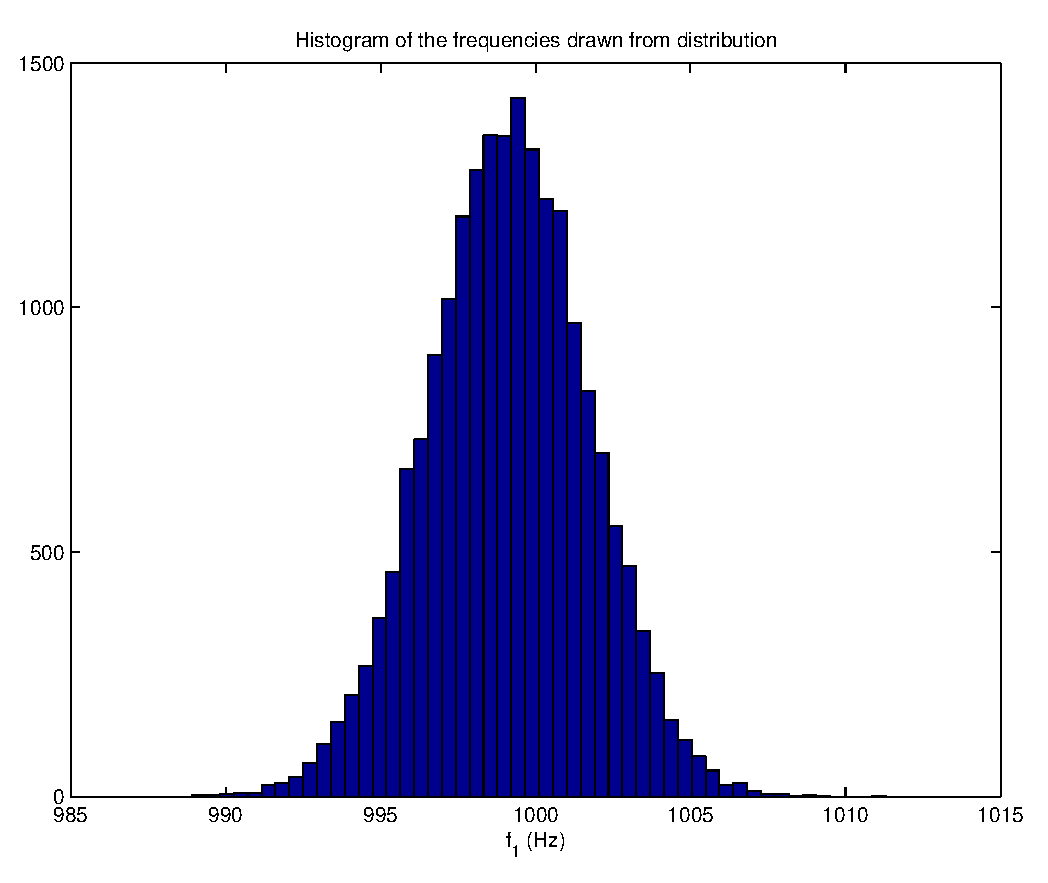
\includegraphics[scale=0.345]{../img3/singleTonewoMHFig12.eps}
			\includegraphics[scale=0.345]{../img3/histWMH.eps}
			\caption{Comparisson of samples drawn from inverse CDF (rigth) and from Metropolis-Hastings (left).}
		\end{figure}
		
		
	\end{frame}
	
	
	
	%========================================================================
	%SECOND SECTION STARTS HERE
	%========================================================================
	\section{Two tone case}
	\subsection{Finding Maximum Likelihood Estimators}
	
	\begin{frame}{Estimating frequencies of two tones}
		The following signal is composed by two complex sinusoids in additive Gaussian white noise.
		
		\begin{equation}
			r(t) = A_{1}e^{j2\pi f_1 t} + A_{2}e^{j2\pi f_2 t} + z(t)
		\end{equation}
	
		\begin{figure}
			\centering
			\includegraphics[scale=0.4]{../img3/2TonewoMHFig1.eps}
		\end{figure}
	\end{frame}
	
	\begin{frame}{Estimating frequencies of two tones}
		Estimating the frequencies of the two tones may be hard. Specially if the two frequencies are close.
		
		The frequencies used in this simulation are $f_1 = 1\mathrm{kHz}$ and $f_2 = 1.5\mathrm{kHz}$. Amplitudes are $A_1 = 2$ and $A_2 = 2$.
	
		\begin{figure}
			\centering
			\includegraphics[scale=0.3]{../img3/2TonewoMHFig2.eps}
			\includegraphics[scale=0.3]{../img3/2TonewoMHFig3.eps}
			\caption{Discrete-time Fourier Transform and power spectral density of the two sinusoids with added noise.}
		\end{figure}
	\end{frame}
	
	\begin{frame}{Estimating frequencies of two tones}
		Since the two frequencies are very distinct, they won't interfere with each other. The maximum likelihood estimators can be found by maximizing the following function.
		
		\begin{gather*}
			\mathbf{r} =  [r(0) \; \; r(T_s) \; \; r(2T_s) \; \dots \; r((N-1)T_s)]^T \\
			\mathbf{e_i} =  [e^{j2\pi f_i0} \; e^{j2\pi f_iT_s} \; \dots \; e^{j2\pi f_i(N-1)T_s}]^T \\	
			\mathbf{E} = [\mathbf{e_1} \; \mathbf{e_2}]\\
			L(f_1,f_2) = \mathbf{r'E}(\mathbf{E'E})^{-1}\mathbf{E'r} \\
		\end{gather*}
		
	\end{frame}
	
	\begin{frame}{Estimating frequencies of two tones}
		\begin{figure}
			\centering
			\includegraphics[scale=0.5]{../img3/2TonewoMHFig6.eps}
		\end{figure}
	\end{frame}
	\subsection{Defining Probability Density Functions}
	%========================================================================
	%I START TO TALK ABOUT PDFS FOR THE TWO TONE CASE HERE
	%========================================================================
	\begin{frame}{Conditioned PDF of the frequencies}
		\begin{gather*}
			\mathbf{r} =  [r(0) \; \; r(T_s) \; \; r(2T_s) \; \dots \; r((N-1)T_s)]^T \\
			\mathbf{e_i} =  [e^{j2\pi f_i0} \; e^{j2\pi f_iT_s} \; \dots \; e^{j2\pi f_i(N-1)T_s}]^T \\
			\mathbf{r} =  A_1\mathbf{e_1}+A_2\mathbf{e_2}+\mathbf{n}\\
			\mathbf{y} =\mathbf{r} - A_2\mathbf{e_2}\\
			\mathrm{p}(\mathbf{r}|f_1,f_2,A_1,A_2) = \frac{1}{\pi^N\sigma^{2N}}
			\exp\left[-\frac{(\mathbf{y}-A_1\mathbf{e_1})'(\mathbf{y}-A_1\mathbf{e_1})}{\sigma^2}\right] \\
			\mathrm{p}(\mathbf{r}|f_2,A_1,A_2) = \int \mathrm{p}(\mathbf{r}|f_1,f_2,A_1,A_2)\mathrm{p}(f_1)df_1\\
			\mathrm{p}(f_1|\mathbf{r},f_2,A_1,A_2) = \frac{\mathrm{p}(\mathbf{r}|f_1,f_2,A_1,A_2)\mathrm{p}(f_1)}{\mathrm{p}(\mathbf{r}|f_2,A_1,A_2)} \\
		\end{gather*}
	\end{frame}
	
	\begin{frame}{Conditioned PDF of the frequencies}
		\begin{figure}
			\centering
			\includegraphics[scale=0.33]{../img3/2TonewoMHFig7.eps}
			\includegraphics[scale=0.33]{../img3/2TonewoMHFig8.eps}
			\caption{PDF's of the frequencies conditioned on the MLE's of the other parameters. All the values on the top of the plots were estimated from data.}
		\end{figure}
	\end{frame}
	
	\begin{frame}{Conditioned PDF of the amplitudes}
		Calculating the PDF of the amplitudes require some trivial operation with random vectors.
		\begin{gather*}
			\mathbf{r} =  A_1\mathbf{e_1}+A_2\mathbf{e_2}+\mathbf{n}\\
			\mathbf{e_1'r} = A_1N+A_2\mathbf{e_1'e_2}+\mathbf{e_1'n}\\
			A_1 = \frac{\mathbf{e_1'r}-A_2\mathbf{e_1'e_2}-\mathbf{e_1'n}}{N}\\
			A_1|\mathbf{r},f_1,f_2,A_2 \sim \mathcal{N}\left(\frac{\mathbf{e_1'r}-A_2\mathbf{e_1'e_2}}{N},\frac{\sigma^2}{N}\right)
		\end{gather*}
		Replace $\mathbf{e_1'}$ with $\mathbf{e_2'}$ in the second line to get the PDF of $A_2$. Note that the mean of the distribution is complex.
		
	\end{frame}
	
	\begin{frame}{Conditioned PDF of the amplitudes}
		\begin{figure}
			\centering
			\includegraphics[scale=0.345]{../img3/2TonewoMHFig4.eps}
			\includegraphics[scale=0.345]{../img3/2TonewoMHFig5.eps}
			\caption{PDF's of the amplitudes conditioned on the MLE's of the other parameters. All the values on the top of the plots were estimated from data.}
		\end{figure}
	\end{frame}
	
	\begin{frame}{Markov Chain Monte Carlo algorithm}
		\begin{algorithm}[H]
			\For{n = 2:Nmcmc}{
			Asamp1[n] = Sample of $A_1$ conditioned on Asamp2[n-1], fsamp1[n-1] and fsamp2[n-1];\\
			Asamp2[n] = Sample of $A_2$ conditioned on Asamp1[n-1], fsamp1[n-1] and fsamp2[n-1];\\			
			fsamp1[n] = Sample of $f_1$ conditioned on Asamp1[n], Asamp2[n] and fsamp2[n-1];\\			
			fsamp2[n] = Sample of $f_2$ conditioned on Asamp1[n], Asamp2[n] and fsamp1[n-1];\\
			}
		\end{algorithm}
	\end{frame}
	
	\begin{frame}{Unconditioned PDF from MCMC}
		\begin{figure}
			\centering
			\includegraphics[scale=0.33]{../img3/2TonewoMHFig11.eps}
			\includegraphics[scale=0.33]{../img3/2TonewoMHFig12.eps}
			\caption{PDF's of the frequencies conditioned just on the data. They were obtained using the Markov Chain Monte Carlo method to draw samples from distributions.}
		\end{figure}
	\end{frame}
	
	\begin{frame}{Unconditioned PDF from MCMC}
		\begin{figure}
			\centering
			\includegraphics[scale=0.345]{../img3/2TonewoMHFig9.eps}
			\includegraphics[scale=0.345]{../img3/2TonewoMHFig10.eps}
			\caption{PDF's of the amplitudes conditioned just on the data. They were obtained using the Markov Chain Monte Carlo method to draw samples from distributions.}
		\end{figure}
	\end{frame}
	
	\begin{frame}{Unconditioned PDF from MCMC}
		\begin{figure}
			\centering
			\includegraphics[scale=0.45]{../img3/2TonewoMHFig13.eps}
		\end{figure}
	\end{frame}
	%========================================================================
	%LAST SECTION STARTS HERE
	%========================================================================
	\section{Future Work}
	
	\begin{frame}{Future work}
		\begin{itemize}
			\item Apply the Metropolis-Hastings algorithm to estimate the PDF's of the frequencies and amplitude in the two-tone case.
			
			\item Find a faster way to run the Markov Chain Monte Carlo algorithm.
			
			\item Have a better understanding of how the estimation works
			
		\end{itemize}
	\end{frame}
	

	
\end{document}